\documentclass[1p]{elsarticle_modified}
%\bibliographystyle{elsarticle-num}

%\usepackage[colorlinks]{hyperref}
%\usepackage{abbrmath_seonhwa} %\Abb, \Ascr, \Acal ,\Abf, \Afrak
\usepackage{amsfonts}
\usepackage{amssymb}
\usepackage{amsmath}
\usepackage{amsthm}
\usepackage{scalefnt}
\usepackage{amsbsy}
\usepackage{kotex}
\usepackage{caption}
\usepackage{subfig}
\usepackage{color}
\usepackage{graphicx}
\usepackage{xcolor} %% white, black, red, green, blue, cyan, magenta, yellow
\usepackage{float}
\usepackage{setspace}
\usepackage{hyperref}

\usepackage{tikz}
\usetikzlibrary{arrows}

\usepackage{multirow}
\usepackage{array} % fixed length table
\usepackage{hhline}

%%%%%%%%%%%%%%%%%%%%%
\makeatletter
\renewcommand*\env@matrix[1][\arraystretch]{%
	\edef\arraystretch{#1}%
	\hskip -\arraycolsep
	\let\@ifnextchar\new@ifnextchar
	\array{*\c@MaxMatrixCols c}}
\makeatother %https://tex.stackexchange.com/questions/14071/how-can-i-increase-the-line-spacing-in-a-matrix
%%%%%%%%%%%%%%%

\usepackage[normalem]{ulem}

\newcommand{\msout}[1]{\ifmmode\text{\sout{\ensuremath{#1}}}\else\sout{#1}\fi}
%SOURCE: \msout is \stkout macro in https://tex.stackexchange.com/questions/20609/strikeout-in-math-mode

\newcommand{\cancel}[1]{
	\ifmmode
	{\color{red}\msout{#1}}
	\else
	{\color{red}\sout{#1}}
	\fi
}

\newcommand{\add}[1]{
	{\color{blue}\uwave{#1}}
}

\newcommand{\replace}[2]{
	\ifmmode
	{\color{red}\msout{#1}}{\color{blue}\uwave{#2}}
	\else
	{\color{red}\sout{#1}}{\color{blue}\uwave{#2}}
	\fi
}

\newcommand{\Sol}{\mathcal{S}} %segment
\newcommand{\D}{D} %diagram
\newcommand{\A}{\mathcal{A}} %arc


%%%%%%%%%%%%%%%%%%%%%%%%%%%%%5 test

\def\sl{\operatorname{\textup{SL}}(2,\Cbb)}
\def\psl{\operatorname{\textup{PSL}}(2,\Cbb)}
\def\quan{\mkern 1mu \triangleright \mkern 1mu}

\theoremstyle{definition}
\newtheorem{thm}{Theorem}[section]
\newtheorem{prop}[thm]{Proposition}
\newtheorem{lem}[thm]{Lemma}
\newtheorem{ques}[thm]{Question}
\newtheorem{cor}[thm]{Corollary}
\newtheorem{defn}[thm]{Definition}
\newtheorem{exam}[thm]{Example}
\newtheorem{rmk}[thm]{Remark}
\newtheorem{alg}[thm]{Algorithm}

\newcommand{\I}{\sqrt{-1}}
\begin{document}

%\begin{frontmatter}
%
%\title{Boundary parabolic representations of knots up to 8 crossings}
%
%%% Group authors per affiliation:
%\author{Yunhi Cho} 
%\address{Department of Mathematics, University of Seoul, Seoul, Korea}
%\ead{yhcho@uos.ac.kr}
%
%
%\author{Seonhwa Kim} %\fnref{s_kim}}
%\address{Center for Geometry and Physics, Institute for Basic Science, Pohang, 37673, Korea}
%\ead{ryeona17@ibs.re.kr}
%
%\author{Hyuk Kim}
%\address{Department of Mathematical Sciences, Seoul National University, Seoul 08826, Korea}
%\ead{hyukkim@snu.ac.kr}
%
%\author{Seokbeom Yoon}
%\address{Department of Mathematical Sciences, Seoul National University, Seoul, 08826,  Korea}
%\ead{sbyoon15@snu.ac.kr}
%
%\begin{abstract}
%We find all boundary parabolic representation of knots up to 8 crossings.
%
%\end{abstract}
%\begin{keyword}
%    \MSC[2010] 57M25 
%\end{keyword}
%
%\end{frontmatter}

%\linenumbers
%\tableofcontents
%
\newcommand\colored[1]{\textcolor{white}{\rule[-0.35ex]{0.8em}{1.4ex}}\kern-0.8em\color{red} #1}%
%\newcommand\colored[1]{\textcolor{white}{ #1}\kern-2.17ex	\textcolor{white}{ #1}\kern-1.81ex	\textcolor{white}{ #1}\kern-2.15ex\color{red}#1	}

{\Large $\underline{12n_{0509}~(K12n_{0509})}$}

\setlength{\tabcolsep}{10pt}
\renewcommand{\arraystretch}{1.6}
\vspace{1cm}\begin{tabular}{m{100pt}>{\centering\arraybackslash}m{274pt}}
\multirow{5}{120pt}{
	\centering
	\includegraphics[width=112pt]{../../../GIT/diagram.site/Diagrams/png/2598_12n_0509.png}\\
\ \ \ A knot diagram\footnotemark}&
\allowdisplaybreaks
\textbf{Linearized knot diagam} \\
\cline{2-2}
 &
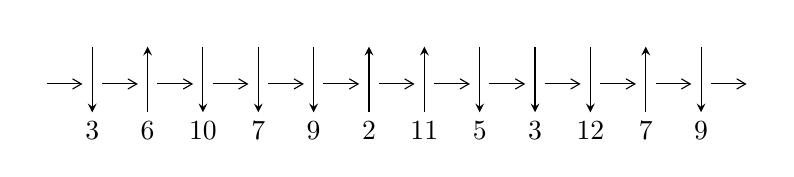
\begin{tikzpicture}[x=20pt, y=17pt]
	% nodes
	\node (C0) at (0, 0) {};
	\node (C1) at (1, 0) {};
	\node (C1U) at (1, +1) {};
	\node (C1D) at (1, -1) {3};

	\node (C2) at (2, 0) {};
	\node (C2U) at (2, +1) {};
	\node (C2D) at (2, -1) {6};

	\node (C3) at (3, 0) {};
	\node (C3U) at (3, +1) {};
	\node (C3D) at (3, -1) {10};

	\node (C4) at (4, 0) {};
	\node (C4U) at (4, +1) {};
	\node (C4D) at (4, -1) {7};

	\node (C5) at (5, 0) {};
	\node (C5U) at (5, +1) {};
	\node (C5D) at (5, -1) {9};

	\node (C6) at (6, 0) {};
	\node (C6U) at (6, +1) {};
	\node (C6D) at (6, -1) {2};

	\node (C7) at (7, 0) {};
	\node (C7U) at (7, +1) {};
	\node (C7D) at (7, -1) {11};

	\node (C8) at (8, 0) {};
	\node (C8U) at (8, +1) {};
	\node (C8D) at (8, -1) {5};

	\node (C9) at (9, 0) {};
	\node (C9U) at (9, +1) {};
	\node (C9D) at (9, -1) {3};

	\node (C10) at (10, 0) {};
	\node (C10U) at (10, +1) {};
	\node (C10D) at (10, -1) {12};

	\node (C11) at (11, 0) {};
	\node (C11U) at (11, +1) {};
	\node (C11D) at (11, -1) {7};

	\node (C12) at (12, 0) {};
	\node (C12U) at (12, +1) {};
	\node (C12D) at (12, -1) {9};
	\node (C13) at (13, 0) {};

	% arrows
	\draw[->,>={angle 60}]
	(C0) edge (C1) (C1) edge (C2) (C2) edge (C3) (C3) edge (C4) (C4) edge (C5) (C5) edge (C6) (C6) edge (C7) (C7) edge (C8) (C8) edge (C9) (C9) edge (C10) (C10) edge (C11) (C11) edge (C12) (C12) edge (C13) ;	\draw[->,>=stealth]
	(C1U) edge (C1D) (C2D) edge (C2U) (C3U) edge (C3D) (C4U) edge (C4D) (C5U) edge (C5D) (C6D) edge (C6U) (C7D) edge (C7U) (C8U) edge (C8D) (C9U) edge (C9D) (C10U) edge (C10D) (C11D) edge (C11U) (C12U) edge (C12D) ;
	\end{tikzpicture} \\
\hhline{~~} \\& 
\textbf{Solving Sequence} \\ \cline{2-2} 
 &
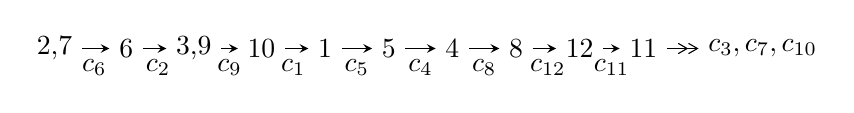
\begin{tikzpicture}[x=23pt, y=7pt]
	% node
	\node (A0) at (-1/8, 0) {2,7};
	\node (A1) at (1, 0) {6};
	\node (A2) at (33/16, 0) {3,9};
	\node (A3) at (25/8, 0) {10};
	\node (A4) at (33/8, 0) {1};
	\node (A5) at (41/8, 0) {5};
	\node (A6) at (49/8, 0) {4};
	\node (A7) at (57/8, 0) {8};
	\node (A8) at (65/8, 0) {12};
	\node (A9) at (73/8, 0) {11};
	\node (C1) at (1/2, -1) {$c_{6}$};
	\node (C2) at (3/2, -1) {$c_{2}$};
	\node (C3) at (21/8, -1) {$c_{9}$};
	\node (C4) at (29/8, -1) {$c_{1}$};
	\node (C5) at (37/8, -1) {$c_{5}$};
	\node (C6) at (45/8, -1) {$c_{4}$};
	\node (C7) at (53/8, -1) {$c_{8}$};
	\node (C8) at (61/8, -1) {$c_{12}$};
	\node (C9) at (69/8, -1) {$c_{11}$};
	\node (A10) at (11, 0) {$c_{3},c_{7},c_{10}$};

	% edge
	\draw[->,>=stealth]	
	(A0) edge (A1) (A1) edge (A2) (A2) edge (A3) (A3) edge (A4) (A4) edge (A5) (A5) edge (A6) (A6) edge (A7) (A7) edge (A8) (A8) edge (A9) ;
	\draw[->>,>={angle 60}]	
	(A9) edge (A10);
\end{tikzpicture} \\ 

\end{tabular} \\

\footnotetext{
The image of knot diagram is generated by the software ``\textbf{Draw programme}" developed by Andrew Bartholomew(\url{http://www.layer8.co.uk/maths/draw/index.htm\#Running-draw}), where we modified some parts for our purpose(\url{https://github.com/CATsTAILs/LinksPainter}).
}\phantom \\ \newline 
\centering \textbf{Ideals for irreducible components\footnotemark of $X_{\text{par}}$} 
 
\begin{align*}
I^u_{1}&=\langle 
- u^6+3 u^5-6 u^4+7 u^3-6 u^2+b+3 u-1,\;u^6-3 u^5+6 u^4-7 u^3+5 u^2+a-3 u,\\
\phantom{I^u_{1}}&\phantom{= \langle  }u^7-3 u^6+7 u^5-10 u^4+10 u^3-8 u^2+3 u-1\rangle \\
I^u_{2}&=\langle 
-3 u^{13}+14 u^{12}+\cdots+4 b+4,\;u^{13}-8 u^{12}+\cdots+8 a-4,\;u^{14}-6 u^{13}+\cdots-28 u+8\rangle \\
I^u_{3}&=\langle 
- u^2+b+a-1,\;a^2+a u+2 u^2- a+u,\;u^3+u^2+2 u+1\rangle \\
I^u_{4}&=\langle 
- u^6- u^5-2 u^4- u^3-2 u^2+b- u-1,\;u^6+u^5+2 u^4+u^3+3 u^2+a+u+2,\\
\phantom{I^u_{4}}&\phantom{= \langle  }u^7+u^6+3 u^5+2 u^4+4 u^3+2 u^2+3 u+1\rangle \\
I^u_{5}&=\langle 
-2 u^2 a- a u-2 u^2+b-2 a- u-4,\;2 u^2 a+a^2+2 u^2+3 a+2 u+4,\;u^3+u^2+2 u+1\rangle \\
I^u_{6}&=\langle 
- u^2 a+2 u^2+2 b+u+3,\;a^2+3 u^2+3 u+2,\;u^3+u^2+2 u+1\rangle \\
I^u_{7}&=\langle 
u^6+u^5+2 u^4+u^3+u^2+b+u+1,\;-2 u^7-2 u^6-5 u^5-3 u^4-3 u^3-3 u^2+a-4 u-1,\\
\phantom{I^u_{7}}&\phantom{= \langle  }u^8+u^7+3 u^6+2 u^5+3 u^4+2 u^3+3 u^2+u+1\rangle \\
\\
\end{align*}
\raggedright * 7 irreducible components of $\dim_{\mathbb{C}}=0$, with total 54 representations.\\
\footnotetext{All coefficients of polynomials are rational numbers. But the coefficients are sometimes approximated in decimal forms when there is not enough margin.}
\newpage
\renewcommand{\arraystretch}{1}
\centering \section*{I. $I^u_{1}= \langle - u^6+3 u^5-6 u^4+7 u^3-6 u^2+b+3 u-1,\;u^6-3 u^5+6 u^4-7 u^3+5 u^2+a-3 u,\;u^7-3 u^6+7 u^5-10 u^4+10 u^3-8 u^2+3 u-1 \rangle$}
\flushleft \textbf{(i) Arc colorings}\\
\begin{tabular}{m{7pt} m{180pt} m{7pt} m{180pt} }
\flushright $a_{2}=$&$\begin{pmatrix}0\\u\end{pmatrix}$ \\
\flushright $a_{7}=$&$\begin{pmatrix}1\\0\end{pmatrix}$ \\
\flushright $a_{6}=$&$\begin{pmatrix}1\\u^2\end{pmatrix}$ \\
\flushright $a_{3}=$&$\begin{pmatrix}u\\u^3+u\end{pmatrix}$ \\
\flushright $a_{9}=$&$\begin{pmatrix}- u^6+3 u^5-6 u^4+7 u^3-5 u^2+3 u\\u^6-3 u^5+6 u^4-7 u^3+6 u^2-3 u+1\end{pmatrix}$ \\
\flushright $a_{10}=$&$\begin{pmatrix}- u^6+2 u^5-4 u^4+4 u^3-3 u^2+2 u\\- u^3- u\end{pmatrix}$ \\
\flushright $a_{1}=$&$\begin{pmatrix}u^3\\u^5+u^3+u\end{pmatrix}$ \\
\flushright $a_{5}=$&$\begin{pmatrix}- u^5+2 u^4-3 u^3+3 u^2- u+1\\- u^6+3 u^5-6 u^4+7 u^3-6 u^2+3 u-1\end{pmatrix}$ \\
\flushright $a_{4}=$&$\begin{pmatrix}- u^6+2 u^5-4 u^4+4 u^3-3 u^2+2 u\\- u^6+3 u^5-6 u^4+7 u^3-6 u^2+3 u-1\end{pmatrix}$ \\
\flushright $a_{8}=$&$\begin{pmatrix}- u^6+2 u^5-4 u^4+4 u^3- u^2+u+1\\- u^2\end{pmatrix}$ \\
\flushright $a_{12}=$&$\begin{pmatrix}u^5-2 u^4+4 u^3-4 u^2+2 u-1\\u\end{pmatrix}$ \\
\flushright $a_{11}=$&$\begin{pmatrix}u^5-2 u^4+4 u^3-4 u^2+u-1\\u\end{pmatrix}$\\&\end{tabular}
\flushleft \textbf{(ii) Obstruction class $= -1$}\\~\\
\flushleft \textbf{(iii) Cusp Shapes $= 2 u^6-8 u^5+20 u^4-32 u^3+36 u^2-30 u+5$}\\~\\
\newpage\renewcommand{\arraystretch}{1}
\flushleft \textbf{(iv) u-Polynomials at the component}\newline \\
\begin{tabular}{m{50pt}|m{274pt}}
Crossings & \hspace{64pt}u-Polynomials at each crossing \\
\hline $$\begin{aligned}c_{1},c_{10}\end{aligned}$$&$\begin{aligned}
&u^7+5 u^6+9 u^5-2 u^4-24 u^3-24 u^2-7 u-1
\end{aligned}$\\
\hline $$\begin{aligned}c_{2},c_{6},c_{7}\\c_{11}\end{aligned}$$&$\begin{aligned}
&u^7-3 u^6+7 u^5-10 u^4+10 u^3-8 u^2+3 u-1
\end{aligned}$\\
\hline $$\begin{aligned}c_{3},c_{5},c_{8}\\c_{9}\end{aligned}$$&$\begin{aligned}
&u^7+5 u^6+8 u^5+4 u^4+2 u^3+5 u^2+3 u+1
\end{aligned}$\\
\hline $$\begin{aligned}c_{4},c_{12}\end{aligned}$$&$\begin{aligned}
&u^7- u^6-8 u^5+5 u^4+21 u^3+14 u^2+4 u+1
\end{aligned}$\\
\hline
\end{tabular}\\~\\
\newpage\renewcommand{\arraystretch}{1}
\flushleft \textbf{(v) Riley Polynomials at the component}\newline \\
\begin{tabular}{m{50pt}|m{274pt}}
Crossings & \hspace{64pt}Riley Polynomials at each crossing \\
\hline $$\begin{aligned}c_{1},c_{10}\end{aligned}$$&$\begin{aligned}
&y^7-7 y^6+53 y^5-210 y^4+364 y^3-244 y^2+y-1
\end{aligned}$\\
\hline $$\begin{aligned}c_{2},c_{6},c_{7}\\c_{11}\end{aligned}$$&$\begin{aligned}
&y^7+5 y^6+9 y^5-2 y^4-24 y^3-24 y^2-7 y-1
\end{aligned}$\\
\hline $$\begin{aligned}c_{3},c_{5},c_{8}\\c_{9}\end{aligned}$$&$\begin{aligned}
&y^7-9 y^6+28 y^5-28 y^4+2 y^3-21 y^2- y-1
\end{aligned}$\\
\hline $$\begin{aligned}c_{4},c_{12}\end{aligned}$$&$\begin{aligned}
&y^7-17 y^6+116 y^5-325 y^4+239 y^3-38 y^2-12 y-1
\end{aligned}$\\
\hline
\end{tabular}\\~\\
\newpage\flushleft \textbf{(vi) Complex Volumes and Cusp Shapes}
$$\begin{array}{c|c|c}  
\text{Solutions to }I^u_{1}& \I (\text{vol} + \sqrt{-1}CS) & \text{Cusp shape}\\
 \hline 
\begin{aligned}
u &= \phantom{-}0.136302 + 1.137730 I \\
a &= -1.052660 + 0.165088 I \\
b &= \phantom{-}0.776815 + 0.145062 I\end{aligned}
 & -4.44698 + 2.33074 I & -9.82174 - 3.80507 I \\ \hline\begin{aligned}
u &= \phantom{-}0.136302 - 1.137730 I \\
a &= -1.052660 - 0.165088 I \\
b &= \phantom{-}0.776815 - 0.145062 I\end{aligned}
 & -4.44698 - 2.33074 I & -9.82174 + 3.80507 I \\ \hline\begin{aligned}
u &= \phantom{-}1.24390\phantom{ +0.000000I} \\
a &= \phantom{-}0.333091\phantom{ +0.000000I} \\
b &= \phantom{-}2.21419\phantom{ +0.000000I}\end{aligned}
 & -11.4456\phantom{ +0.000000I} & -6.73760\phantom{ +0.000000I} \\ \hline\begin{aligned}
u &= \phantom{-}0.194340 + 0.463986 I \\
a &= \phantom{-}0.726250 + 0.493271 I \\
b &= \phantom{-}0.096235 - 0.312929 I\end{aligned}
 & -0.189704 + 0.962753 I & -3.67202 - 7.06800 I \\ \hline\begin{aligned}
u &= \phantom{-}0.194340 - 0.463986 I \\
a &= \phantom{-}0.726250 - 0.493271 I \\
b &= \phantom{-}0.096235 + 0.312929 I\end{aligned}
 & -0.189704 - 0.962753 I & -3.67202 + 7.06800 I \\ \hline\begin{aligned}
u &= \phantom{-}0.54741 + 1.45600 I \\
a &= \phantom{-}1.65987 + 0.82195 I \\
b &= -2.48014 + 0.77211 I\end{aligned}
 & \phantom{-}18.5842 + 12.7630 I & -10.63743 - 5.46514 I \\ \hline\begin{aligned}
u &= \phantom{-}0.54741 - 1.45600 I \\
a &= \phantom{-}1.65987 - 0.82195 I \\
b &= -2.48014 - 0.77211 I\end{aligned}
 & \phantom{-}18.5842 - 12.7630 I & -10.63743 + 5.46514 I\\
 \hline 
 \end{array}$$\newpage\newpage\renewcommand{\arraystretch}{1}
\centering \section*{II. $I^u_{2}= \langle -3 u^{13}+14 u^{12}+\cdots+4 b+4,\;u^{13}-8 u^{12}+\cdots+8 a-4,\;u^{14}-6 u^{13}+\cdots-28 u+8 \rangle$}
\flushleft \textbf{(i) Arc colorings}\\
\begin{tabular}{m{7pt} m{180pt} m{7pt} m{180pt} }
\flushright $a_{2}=$&$\begin{pmatrix}0\\u\end{pmatrix}$ \\
\flushright $a_{7}=$&$\begin{pmatrix}1\\0\end{pmatrix}$ \\
\flushright $a_{6}=$&$\begin{pmatrix}1\\u^2\end{pmatrix}$ \\
\flushright $a_{3}=$&$\begin{pmatrix}u\\u^3+u\end{pmatrix}$ \\
\flushright $a_{9}=$&$\begin{pmatrix}-\frac{1}{8} u^{13}+u^{12}+\cdots-\frac{3}{4} u+\frac{1}{2}\\\frac{3}{4} u^{13}-\frac{7}{2} u^{12}+\cdots+5 u-1\end{pmatrix}$ \\
\flushright $a_{10}=$&$\begin{pmatrix}-\frac{1}{8} u^{13}+\frac{3}{4} u^{11}+\cdots+\frac{21}{4} u-\frac{3}{2}\\-\frac{5}{4} u^{13}+\frac{13}{2} u^{12}+\cdots-17 u+5\end{pmatrix}$ \\
\flushright $a_{1}=$&$\begin{pmatrix}u^3\\u^5+u^3+u\end{pmatrix}$ \\
\flushright $a_{5}=$&$\begin{pmatrix}\frac{1}{8} u^{13}- u^{12}+\cdots+\frac{21}{4} u-1\\\frac{1}{4} u^{13}- u^{12}+\cdots+\frac{13}{2} u-3\end{pmatrix}$ \\
\flushright $a_{4}=$&$\begin{pmatrix}\frac{3}{8} u^{13}-2 u^{12}+\cdots+\frac{47}{4} u-4\\\frac{1}{4} u^{13}- u^{12}+\cdots+\frac{13}{2} u-3\end{pmatrix}$ \\
\flushright $a_{8}=$&$\begin{pmatrix}\frac{5}{8} u^{13}-\frac{13}{4} u^{12}+\cdots+7 u-1\\-\frac{1}{2} u^{13}+\frac{5}{2} u^{12}+\cdots-\frac{13}{2} u+3\end{pmatrix}$ \\
\flushright $a_{12}=$&$\begin{pmatrix}-\frac{1}{8} u^{13}+u^{12}+\cdots-\frac{17}{4} u+1\\\frac{3}{4} u^{13}-4 u^{12}+\cdots+\frac{31}{2} u-5\end{pmatrix}$ \\
\flushright $a_{11}=$&$\begin{pmatrix}-\frac{7}{8} u^{13}+5 u^{12}+\cdots-\frac{79}{4} u+6\\\frac{3}{4} u^{13}-4 u^{12}+\cdots+\frac{31}{2} u-5\end{pmatrix}$\\&\end{tabular}
\flushleft \textbf{(ii) Obstruction class $= -1$}\\~\\
\flushleft \textbf{(iii) Cusp Shapes $= -2 u^{13}+12 u^{12}-43 u^{11}+105 u^{10}-196 u^9+295 u^8-375 u^7+414 u^6-395 u^5+319 u^4-217 u^3+130 u^2-70 u+18$}\\~\\
\newpage\renewcommand{\arraystretch}{1}
\flushleft \textbf{(iv) u-Polynomials at the component}\newline \\
\begin{tabular}{m{50pt}|m{274pt}}
Crossings & \hspace{64pt}u-Polynomials at each crossing \\
\hline $$\begin{aligned}c_{1},c_{10}\end{aligned}$$&$\begin{aligned}
&u^{14}+8 u^{13}+\cdots+240 u+64
\end{aligned}$\\
\hline $$\begin{aligned}c_{2},c_{6},c_{7}\\c_{11}\end{aligned}$$&$\begin{aligned}
&u^{14}-6 u^{13}+\cdots-28 u+8
\end{aligned}$\\
\hline $$\begin{aligned}c_{3},c_{5},c_{8}\\c_{9}\end{aligned}$$&$\begin{aligned}
&(u^7-2 u^6-3 u^5+7 u^4-3 u^2+1)^2
\end{aligned}$\\
\hline $$\begin{aligned}c_{4},c_{12}\end{aligned}$$&$\begin{aligned}
&u^{14}-2 u^{13}+\cdots+15 u+1
\end{aligned}$\\
\hline
\end{tabular}\\~\\
\newpage\renewcommand{\arraystretch}{1}
\flushleft \textbf{(v) Riley Polynomials at the component}\newline \\
\begin{tabular}{m{50pt}|m{274pt}}
Crossings & \hspace{64pt}Riley Polynomials at each crossing \\
\hline $$\begin{aligned}c_{1},c_{10}\end{aligned}$$&$\begin{aligned}
&y^{14}+72 y^{12}+\cdots+13056 y+4096
\end{aligned}$\\
\hline $$\begin{aligned}c_{2},c_{6},c_{7}\\c_{11}\end{aligned}$$&$\begin{aligned}
&y^{14}+8 y^{13}+\cdots+240 y+64
\end{aligned}$\\
\hline $$\begin{aligned}c_{3},c_{5},c_{8}\\c_{9}\end{aligned}$$&$\begin{aligned}
&(y^7-10 y^6+37 y^5-61 y^4+46 y^3-23 y^2+6 y-1)^2
\end{aligned}$\\
\hline $$\begin{aligned}c_{4},c_{12}\end{aligned}$$&$\begin{aligned}
&y^{14}-24 y^{13}+\cdots-53 y+1
\end{aligned}$\\
\hline
\end{tabular}\\~\\
\newpage\flushleft \textbf{(vi) Complex Volumes and Cusp Shapes}
$$\begin{array}{c|c|c}  
\text{Solutions to }I^u_{2}& \I (\text{vol} + \sqrt{-1}CS) & \text{Cusp shape}\\
 \hline 
\begin{aligned}
u &= \phantom{-}0.625244 + 0.634655 I \\
a &= \phantom{-}0.339092 + 0.351980 I \\
b &= \phantom{-}0.233020 - 0.022062 I\end{aligned}
 & \phantom{-}0.091886 + 0.891330 I & -6.03895 - 5.74662 I \\ \hline\begin{aligned}
u &= \phantom{-}0.625244 - 0.634655 I \\
a &= \phantom{-}0.339092 - 0.351980 I \\
b &= \phantom{-}0.233020 + 0.022062 I\end{aligned}
 & \phantom{-}0.091886 - 0.891330 I & -6.03895 + 5.74662 I \\ \hline\begin{aligned}
u &= -0.378126 + 1.062500 I \\
a &= -1.121480 - 0.077660 I \\
b &= \phantom{-}0.404958 + 1.328870 I\end{aligned}
 & -1.03722 - 4.17104 I & -10.56067 + 2.18298 I \\ \hline\begin{aligned}
u &= -0.378126 - 1.062500 I \\
a &= -1.121480 + 0.077660 I \\
b &= \phantom{-}0.404958 - 1.328870 I\end{aligned}
 & -1.03722 + 4.17104 I & -10.56067 - 2.18298 I \\ \hline\begin{aligned}
u &= \phantom{-}0.643460 + 1.009790 I \\
a &= -0.104502 - 0.643158 I \\
b &= \phantom{-}0.260752 - 0.097466 I\end{aligned}
 & -1.03722 + 4.17104 I & -10.56067 - 2.18298 I \\ \hline\begin{aligned}
u &= \phantom{-}0.643460 - 1.009790 I \\
a &= -0.104502 + 0.643158 I \\
b &= \phantom{-}0.260752 + 0.097466 I\end{aligned}
 & -1.03722 - 4.17104 I & -10.56067 + 2.18298 I \\ \hline\begin{aligned}
u &= \phantom{-}1.204680 + 0.069237 I \\
a &= -0.311651 - 0.047691 I \\
b &= -2.19150 + 0.08443 I\end{aligned}
 & -16.0632 + 6.5463 I & -8.56192 - 3.00206 I \\ \hline\begin{aligned}
u &= \phantom{-}1.204680 - 0.069237 I \\
a &= -0.311651 + 0.047691 I \\
b &= -2.19150 - 0.08443 I\end{aligned}
 & -16.0632 - 6.5463 I & -8.56192 + 3.00206 I \\ \hline\begin{aligned}
u &= -0.321436 + 0.722211 I \\
a &= \phantom{-}1.113680 + 0.162158 I \\
b &= \phantom{-}0.125852 - 0.871897 I\end{aligned}
 & \phantom{-}0.091886 + 0.891330 I & -6.03895 - 5.74662 I \\ \hline\begin{aligned}
u &= -0.321436 - 0.722211 I \\
a &= \phantom{-}1.113680 - 0.162158 I \\
b &= \phantom{-}0.125852 + 0.871897 I\end{aligned}
 & \phantom{-}0.091886 - 0.891330 I & -6.03895 + 5.74662 I\\
 \hline 
 \end{array}$$\newpage$$\begin{array}{c|c|c}  
\text{Solutions to }I^u_{2}& \I (\text{vol} + \sqrt{-1}CS) & \text{Cusp shape}\\
 \hline 
\begin{aligned}
u &= \phantom{-}0.63252 + 1.42544 I \\
a &= \phantom{-}1.28836 + 1.02059 I \\
b &= -2.20148 + 0.65782 I\end{aligned}
 & \phantom{-}19.2127\phantom{ +0.000000I} & -10.67691 + 0. I\phantom{ +0.000000I} \\ \hline\begin{aligned}
u &= \phantom{-}0.63252 - 1.42544 I \\
a &= \phantom{-}1.28836 - 1.02059 I \\
b &= -2.20148 - 0.65782 I\end{aligned}
 & \phantom{-}19.2127\phantom{ +0.000000I} & -10.67691 + 0. I\phantom{ +0.000000I} \\ \hline\begin{aligned}
u &= \phantom{-}0.59366 + 1.46472 I \\
a &= -1.45351 - 0.86882 I \\
b &= \phantom{-}2.36839 - 0.76461 I\end{aligned}
 & -16.0632 + 6.5463 I & -8.56192 - 3.00206 I \\ \hline\begin{aligned}
u &= \phantom{-}0.59366 - 1.46472 I \\
a &= -1.45351 + 0.86882 I \\
b &= \phantom{-}2.36839 + 0.76461 I\end{aligned}
 & -16.0632 - 6.5463 I & -8.56192 + 3.00206 I\\
 \hline 
 \end{array}$$\newpage\newpage\renewcommand{\arraystretch}{1}
\centering \section*{III. $I^u_{3}= \langle - u^2+b+a-1,\;a^2+a u+2 u^2- a+u,\;u^3+u^2+2 u+1 \rangle$}
\flushleft \textbf{(i) Arc colorings}\\
\begin{tabular}{m{7pt} m{180pt} m{7pt} m{180pt} }
\flushright $a_{2}=$&$\begin{pmatrix}0\\u\end{pmatrix}$ \\
\flushright $a_{7}=$&$\begin{pmatrix}1\\0\end{pmatrix}$ \\
\flushright $a_{6}=$&$\begin{pmatrix}1\\u^2\end{pmatrix}$ \\
\flushright $a_{3}=$&$\begin{pmatrix}u\\- u^2- u-1\end{pmatrix}$ \\
\flushright $a_{9}=$&$\begin{pmatrix}a\\u^2- a+1\end{pmatrix}$ \\
\flushright $a_{10}=$&$\begin{pmatrix}u^2 a+a u+2 a- u-1\\u^2+u+1\end{pmatrix}$ \\
\flushright $a_{1}=$&$\begin{pmatrix}- u^2-2 u-1\\u^2+2 u\end{pmatrix}$ \\
\flushright $a_{5}=$&$\begin{pmatrix}u^2 a+a u+u^2+a- u\\- u^2+a-1\end{pmatrix}$ \\
\flushright $a_{4}=$&$\begin{pmatrix}u^2 a+a u+2 a- u-1\\- u^2+a-1\end{pmatrix}$ \\
\flushright $a_{8}=$&$\begin{pmatrix}- u^2 a- a u+3 u^2- a+3 u+2\\- u^2\end{pmatrix}$ \\
\flushright $a_{12}=$&$\begin{pmatrix}- u^2 a+u^2- a- u-1\\u\end{pmatrix}$ \\
\flushright $a_{11}=$&$\begin{pmatrix}- u^2 a+u^2- a-2 u-1\\u\end{pmatrix}$\\&\end{tabular}
\flushleft \textbf{(ii) Obstruction class $= -1$}\\~\\
\flushleft \textbf{(iii) Cusp Shapes $= 8 u^2+8 u+2$}\\~\\
\newpage\renewcommand{\arraystretch}{1}
\flushleft \textbf{(iv) u-Polynomials at the component}\newline \\
\begin{tabular}{m{50pt}|m{274pt}}
Crossings & \hspace{64pt}u-Polynomials at each crossing \\
\hline $$\begin{aligned}c_{1},c_{10}\end{aligned}$$&$\begin{aligned}
&(u^3+3 u^2+2 u-1)^2
\end{aligned}$\\
\hline $$\begin{aligned}c_{2},c_{6},c_{7}\\c_{11}\end{aligned}$$&$\begin{aligned}
&(u^3+u^2+2 u+1)^2
\end{aligned}$\\
\hline $$\begin{aligned}c_{3},c_{5},c_{8}\\c_{9}\end{aligned}$$&$\begin{aligned}
&u^6+u^5-2 u^4+5 u^3+14 u^2-8
\end{aligned}$\\
\hline $$\begin{aligned}c_{4},c_{12}\end{aligned}$$&$\begin{aligned}
&u^6-4 u^5-3 u^4+14 u^3+14 u^2+2 u-1
\end{aligned}$\\
\hline
\end{tabular}\\~\\
\newpage\renewcommand{\arraystretch}{1}
\flushleft \textbf{(v) Riley Polynomials at the component}\newline \\
\begin{tabular}{m{50pt}|m{274pt}}
Crossings & \hspace{64pt}Riley Polynomials at each crossing \\
\hline $$\begin{aligned}c_{1},c_{10}\end{aligned}$$&$\begin{aligned}
&(y^3-5 y^2+10 y-1)^2
\end{aligned}$\\
\hline $$\begin{aligned}c_{2},c_{6},c_{7}\\c_{11}\end{aligned}$$&$\begin{aligned}
&(y^3+3 y^2+2 y-1)^2
\end{aligned}$\\
\hline $$\begin{aligned}c_{3},c_{5},c_{8}\\c_{9}\end{aligned}$$&$\begin{aligned}
&y^6-5 y^5+22 y^4-97 y^3+228 y^2-224 y+64
\end{aligned}$\\
\hline $$\begin{aligned}c_{4},c_{12}\end{aligned}$$&$\begin{aligned}
&y^6-22 y^5+149 y^4-266 y^3+146 y^2-32 y+1
\end{aligned}$\\
\hline
\end{tabular}\\~\\
\newpage\flushleft \textbf{(vi) Complex Volumes and Cusp Shapes}
$$\begin{array}{c|c|c}  
\text{Solutions to }I^u_{3}& \I (\text{vol} + \sqrt{-1}CS) & \text{Cusp shape}\\
 \hline 
\begin{aligned}
u &= -0.215080 + 1.307140 I \\
a &= -1.276330 - 0.394337 I \\
b &= \phantom{-}0.613967 - 0.167943 I\end{aligned}
 & -10.98310 - 5.65624 I & -13.0195 + 5.9589 I \\ \hline\begin{aligned}
u &= -0.215080 + 1.307140 I \\
a &= \phantom{-}2.49141 - 0.91280 I \\
b &= -3.15376 + 0.35052 I\end{aligned}
 & -10.98310 - 5.65624 I & -13.0195 + 5.9589 I \\ \hline\begin{aligned}
u &= -0.215080 - 1.307140 I \\
a &= -1.276330 + 0.394337 I \\
b &= \phantom{-}0.613967 + 0.167943 I\end{aligned}
 & -10.98310 + 5.65624 I & -13.0195 - 5.9589 I \\ \hline\begin{aligned}
u &= -0.215080 - 1.307140 I \\
a &= \phantom{-}2.49141 + 0.91280 I \\
b &= -3.15376 - 0.35052 I\end{aligned}
 & -10.98310 + 5.65624 I & -13.0195 - 5.9589 I \\ \hline\begin{aligned}
u &= -0.569840\phantom{ +0.000000I} \\
a &= \phantom{-}1.51738\phantom{ +0.000000I} \\
b &= -0.192667\phantom{ +0.000000I}\end{aligned}
 & -2.70789\phantom{ +0.000000I} & \phantom{-}0.0390210\phantom{ +0.000000I} \\ \hline\begin{aligned}
u &= -0.569840\phantom{ +0.000000I} \\
a &= \phantom{-}0.0524558\phantom{ +0.000000I} \\
b &= \phantom{-}1.27226\phantom{ +0.000000I}\end{aligned}
 & -2.70789\phantom{ +0.000000I} & \phantom{-}0.0390210\phantom{ +0.000000I}\\
 \hline 
 \end{array}$$\newpage\newpage\renewcommand{\arraystretch}{1}
\centering \section*{IV. $I^u_{4}= \langle - u^6- u^5-2 u^4- u^3-2 u^2+b- u-1,\;u^6+u^5+2 u^4+u^3+3 u^2+a+u+2,\;u^7+u^6+3 u^5+2 u^4+4 u^3+2 u^2+3 u+1 \rangle$}
\flushleft \textbf{(i) Arc colorings}\\
\begin{tabular}{m{7pt} m{180pt} m{7pt} m{180pt} }
\flushright $a_{2}=$&$\begin{pmatrix}0\\u\end{pmatrix}$ \\
\flushright $a_{7}=$&$\begin{pmatrix}1\\0\end{pmatrix}$ \\
\flushright $a_{6}=$&$\begin{pmatrix}1\\u^2\end{pmatrix}$ \\
\flushright $a_{3}=$&$\begin{pmatrix}u\\u^3+u\end{pmatrix}$ \\
\flushright $a_{9}=$&$\begin{pmatrix}- u^6- u^5-2 u^4- u^3-3 u^2- u-2\\u^6+u^5+2 u^4+u^3+2 u^2+u+1\end{pmatrix}$ \\
\flushright $a_{10}=$&$\begin{pmatrix}- u^6-2 u^4-3 u^2-2\\- u^3- u\end{pmatrix}$ \\
\flushright $a_{1}=$&$\begin{pmatrix}u^3\\u^5+u^3+u\end{pmatrix}$ \\
\flushright $a_{5}=$&$\begin{pmatrix}2 u^6+u^5+4 u^4+u^3+5 u^2+u+3\\- u^6- u^5-2 u^4- u^3-2 u^2- u-1\end{pmatrix}$ \\
\flushright $a_{4}=$&$\begin{pmatrix}u^6+2 u^4+3 u^2+2\\- u^6- u^5-2 u^4- u^3-2 u^2- u-1\end{pmatrix}$ \\
\flushright $a_{8}=$&$\begin{pmatrix}u^6+2 u^4+3 u^2- u+1\\- u^2\end{pmatrix}$ \\
\flushright $a_{12}=$&$\begin{pmatrix}u^5+2 u^3+2 u-1\\- u\end{pmatrix}$ \\
\flushright $a_{11}=$&$\begin{pmatrix}u^5+2 u^3+3 u-1\\- u\end{pmatrix}$\\&\end{tabular}
\flushleft \textbf{(ii) Obstruction class $= 1$}\\~\\
\flushleft \textbf{(iii) Cusp Shapes $= 2 u^6-4 u^3-4 u^2-2 u-11$}\\~\\
\newpage\renewcommand{\arraystretch}{1}
\flushleft \textbf{(iv) u-Polynomials at the component}\newline \\
\begin{tabular}{m{50pt}|m{274pt}}
Crossings & \hspace{64pt}u-Polynomials at each crossing \\
\hline $$\begin{aligned}c_{1},c_{10}\end{aligned}$$&$\begin{aligned}
&u^7-5 u^6+13 u^5-22 u^4+24 u^3-16 u^2+5 u+1
\end{aligned}$\\
\hline $$\begin{aligned}c_{2},c_{7}\end{aligned}$$&$\begin{aligned}
&u^7- u^6+3 u^5-2 u^4+4 u^3-2 u^2+3 u-1
\end{aligned}$\\
\hline $$\begin{aligned}c_{3},c_{8}\end{aligned}$$&$\begin{aligned}
&u^7+u^6-4 u^5-4 u^4+6 u^3+3 u^2-3 u+1
\end{aligned}$\\
\hline $$\begin{aligned}c_{4}\end{aligned}$$&$\begin{aligned}
&u^7+u^6- u^4+3 u^3-4 u^2+2 u-1
\end{aligned}$\\
\hline $$\begin{aligned}c_{5},c_{9}\end{aligned}$$&$\begin{aligned}
&u^7- u^6-4 u^5+4 u^4+6 u^3-3 u^2-3 u-1
\end{aligned}$\\
\hline $$\begin{aligned}c_{6},c_{11}\end{aligned}$$&$\begin{aligned}
&u^7+u^6+3 u^5+2 u^4+4 u^3+2 u^2+3 u+1
\end{aligned}$\\
\hline $$\begin{aligned}c_{12}\end{aligned}$$&$\begin{aligned}
&u^7- u^6+u^4+3 u^3+4 u^2+2 u+1
\end{aligned}$\\
\hline
\end{tabular}\\~\\
\newpage\renewcommand{\arraystretch}{1}
\flushleft \textbf{(v) Riley Polynomials at the component}\newline \\
\begin{tabular}{m{50pt}|m{274pt}}
Crossings & \hspace{64pt}Riley Polynomials at each crossing \\
\hline $$\begin{aligned}c_{1},c_{10}\end{aligned}$$&$\begin{aligned}
&y^7+y^6-3 y^5-10 y^4+12 y^3+28 y^2+57 y-1
\end{aligned}$\\
\hline $$\begin{aligned}c_{2},c_{6},c_{7}\\c_{11}\end{aligned}$$&$\begin{aligned}
&y^7+5 y^6+13 y^5+22 y^4+24 y^3+16 y^2+5 y-1
\end{aligned}$\\
\hline $$\begin{aligned}c_{3},c_{5},c_{8}\\c_{9}\end{aligned}$$&$\begin{aligned}
&y^7-9 y^6+36 y^5-76 y^4+82 y^3-37 y^2+3 y-1
\end{aligned}$\\
\hline $$\begin{aligned}c_{4},c_{12}\end{aligned}$$&$\begin{aligned}
&y^7- y^6+8 y^5+11 y^4+3 y^3-6 y^2-4 y-1
\end{aligned}$\\
\hline
\end{tabular}\\~\\
\newpage\flushleft \textbf{(vi) Complex Volumes and Cusp Shapes}
$$\begin{array}{c|c|c}  
\text{Solutions to }I^u_{4}& \I (\text{vol} + \sqrt{-1}CS) & \text{Cusp shape}\\
 \hline 
\begin{aligned}
u &= \phantom{-}0.537424 + 0.962927 I \\
a &= -0.662429 - 0.173919 I \\
b &= \phantom{-}0.300834 - 0.861081 I\end{aligned}
 & -0.10098 + 4.46523 I & -0.57946 - 5.51833 I \\ \hline\begin{aligned}
u &= \phantom{-}0.537424 - 0.962927 I \\
a &= -0.662429 + 0.173919 I \\
b &= \phantom{-}0.300834 + 0.861081 I\end{aligned}
 & -0.10098 - 4.46523 I & -0.57946 + 5.51833 I \\ \hline\begin{aligned}
u &= -0.132251 + 1.213860 I \\
a &= \phantom{-}1.92214 - 0.71131 I \\
b &= -1.46616 + 1.03238 I\end{aligned}
 & -10.69670 - 3.59676 I & -12.51315 + 1.73858 I \\ \hline\begin{aligned}
u &= -0.132251 - 1.213860 I \\
a &= \phantom{-}1.92214 + 0.71131 I \\
b &= -1.46616 - 1.03238 I\end{aligned}
 & -10.69670 + 3.59676 I & -12.51315 - 1.73858 I \\ \hline\begin{aligned}
u &= -0.723592 + 0.997572 I \\
a &= -0.752025 + 0.832832 I \\
b &= \phantom{-}0.223589 + 0.610838 I\end{aligned}
 & -3.82765 - 5.64420 I & -9.10487 + 5.57424 I \\ \hline\begin{aligned}
u &= -0.723592 - 0.997572 I \\
a &= -0.752025 - 0.832832 I \\
b &= \phantom{-}0.223589 - 0.610838 I\end{aligned}
 & -3.82765 + 5.64420 I & -9.10487 - 5.57424 I \\ \hline\begin{aligned}
u &= -0.363162\phantom{ +0.000000I} \\
a &= -2.01537\phantom{ +0.000000I} \\
b &= \phantom{-}0.883481\phantom{ +0.000000I}\end{aligned}
 & -3.64806\phantom{ +0.000000I} & -10.6050\phantom{ +0.000000I}\\
 \hline 
 \end{array}$$\newpage\newpage\renewcommand{\arraystretch}{1}
\centering \section*{V. $I^u_{5}= \langle -2 u^2 a- a u-2 u^2+b-2 a- u-4,\;2 u^2 a+a^2+2 u^2+3 a+2 u+4,\;u^3+u^2+2 u+1 \rangle$}
\flushleft \textbf{(i) Arc colorings}\\
\begin{tabular}{m{7pt} m{180pt} m{7pt} m{180pt} }
\flushright $a_{2}=$&$\begin{pmatrix}0\\u\end{pmatrix}$ \\
\flushright $a_{7}=$&$\begin{pmatrix}1\\0\end{pmatrix}$ \\
\flushright $a_{6}=$&$\begin{pmatrix}1\\u^2\end{pmatrix}$ \\
\flushright $a_{3}=$&$\begin{pmatrix}u\\- u^2- u-1\end{pmatrix}$ \\
\flushright $a_{9}=$&$\begin{pmatrix}a\\2 u^2 a+a u+2 u^2+2 a+u+4\end{pmatrix}$ \\
\flushright $a_{10}=$&$\begin{pmatrix}u^2 a+a u- u^2+a-1\\u^2 a+a u+u^2+2 a+2\end{pmatrix}$ \\
\flushright $a_{1}=$&$\begin{pmatrix}- u^2-2 u-1\\u^2+2 u\end{pmatrix}$ \\
\flushright $a_{5}=$&$\begin{pmatrix}u^2 a+4 u^2+2 a+2 u+7\\- u^2 a-2 u^2-2 a-2 u-4\end{pmatrix}$ \\
\flushright $a_{4}=$&$\begin{pmatrix}2 u^2+3\\- u^2 a-2 u^2-2 a-2 u-4\end{pmatrix}$ \\
\flushright $a_{8}=$&$\begin{pmatrix}4 u^2 a+2 a u+8 u^2+8 a+3 u+14\\u^2 a+2 u^2+a+u+4\end{pmatrix}$ \\
\flushright $a_{12}=$&$\begin{pmatrix}u^2 a+u^2+2 a+1\\2 u^2 a+a u+3 u^2+3 a+u+5\end{pmatrix}$ \\
\flushright $a_{11}=$&$\begin{pmatrix}- u^2 a- a u-2 u^2- a- u-4\\2 u^2 a+a u+3 u^2+3 a+u+5\end{pmatrix}$\\&\end{tabular}
\flushleft \textbf{(ii) Obstruction class $= -1$}\\~\\
\flushleft \textbf{(iii) Cusp Shapes $= 4 u^2 a+4 a u+8 u^2+8 a+4 u+6$}\\~\\
\newpage\renewcommand{\arraystretch}{1}
\flushleft \textbf{(iv) u-Polynomials at the component}\newline \\
\begin{tabular}{m{50pt}|m{274pt}}
Crossings & \hspace{64pt}u-Polynomials at each crossing \\
\hline $$\begin{aligned}c_{1},c_{10}\end{aligned}$$&$\begin{aligned}
&(u^3+3 u^2+2 u-1)^2
\end{aligned}$\\
\hline $$\begin{aligned}c_{2},c_{6},c_{7}\\c_{11}\end{aligned}$$&$\begin{aligned}
&(u^3+u^2+2 u+1)^2
\end{aligned}$\\
\hline $$\begin{aligned}c_{3},c_{9},c_{12}\end{aligned}$$&$\begin{aligned}
&(u^3- u^2-4 u+5)^2
\end{aligned}$\\
\hline $$\begin{aligned}c_{4}\end{aligned}$$&$\begin{aligned}
&u^6+u^5+6 u^4-3 u^3+10 u^2+8
\end{aligned}$\\
\hline $$\begin{aligned}c_{5},c_{8}\end{aligned}$$&$\begin{aligned}
&(u^3+u^2-1)^2
\end{aligned}$\\
\hline
\end{tabular}\\~\\
\newpage\renewcommand{\arraystretch}{1}
\flushleft \textbf{(v) Riley Polynomials at the component}\newline \\
\begin{tabular}{m{50pt}|m{274pt}}
Crossings & \hspace{64pt}Riley Polynomials at each crossing \\
\hline $$\begin{aligned}c_{1},c_{10}\end{aligned}$$&$\begin{aligned}
&(y^3-5 y^2+10 y-1)^2
\end{aligned}$\\
\hline $$\begin{aligned}c_{2},c_{6},c_{7}\\c_{11}\end{aligned}$$&$\begin{aligned}
&(y^3+3 y^2+2 y-1)^2
\end{aligned}$\\
\hline $$\begin{aligned}c_{3},c_{9},c_{12}\end{aligned}$$&$\begin{aligned}
&(y^3-9 y^2+26 y-25)^2
\end{aligned}$\\
\hline $$\begin{aligned}c_{4}\end{aligned}$$&$\begin{aligned}
&y^6+11 y^5+62 y^4+127 y^3+196 y^2+160 y+64
\end{aligned}$\\
\hline $$\begin{aligned}c_{5},c_{8}\end{aligned}$$&$\begin{aligned}
&(y^3- y^2+2 y-1)^2
\end{aligned}$\\
\hline
\end{tabular}\\~\\
\newpage\flushleft \textbf{(vi) Complex Volumes and Cusp Shapes}
$$\begin{array}{c|c|c}  
\text{Solutions to }I^u_{5}& \I (\text{vol} + \sqrt{-1}CS) & \text{Cusp shape}\\
 \hline 
\begin{aligned}
u &= -0.215080 + 1.307140 I \\
a &= \phantom{-}0.824718 - 0.424452 I \\
b &= -0.732199 + 0.986732 I\end{aligned}
 & -6.84548 - 2.82812 I & -6.49024 + 2.97945 I \\ \hline\begin{aligned}
u &= -0.215080 + 1.307140 I \\
a &= -0.50000 + 1.54901 I \\
b &= \phantom{-}0.94728 - 2.29387 I\end{aligned}
 & -10.9831\phantom{ +0.000000I} & -13.01951 + 0. I\phantom{ +0.000000I} \\ \hline\begin{aligned}
u &= -0.215080 - 1.307140 I \\
a &= \phantom{-}0.824718 + 0.424452 I \\
b &= -0.732199 - 0.986732 I\end{aligned}
 & -6.84548 + 2.82812 I & -6.49024 - 2.97945 I \\ \hline\begin{aligned}
u &= -0.215080 - 1.307140 I \\
a &= -0.50000 - 1.54901 I \\
b &= \phantom{-}0.94728 + 2.29387 I\end{aligned}
 & -10.9831\phantom{ +0.000000I} & -13.01951 + 0. I\phantom{ +0.000000I} \\ \hline\begin{aligned}
u &= -0.569840\phantom{ +0.000000I} \\
a &= -1.82472 + 0.42445 I \\
b &= \phantom{-}0.284920 + 0.882689 I\end{aligned}
 & -6.84548 - 2.82812 I & -6.49024 + 2.97945 I \\ \hline\begin{aligned}
u &= -0.569840\phantom{ +0.000000I} \\
a &= -1.82472 - 0.42445 I \\
b &= \phantom{-}0.284920 - 0.882689 I\end{aligned}
 & -6.84548 + 2.82812 I & -6.49024 - 2.97945 I\\
 \hline 
 \end{array}$$\newpage\newpage\renewcommand{\arraystretch}{1}
\centering \section*{VI. $I^u_{6}= \langle - u^2 a+2 u^2+2 b+u+3,\;a^2+3 u^2+3 u+2,\;u^3+u^2+2 u+1 \rangle$}
\flushleft \textbf{(i) Arc colorings}\\
\begin{tabular}{m{7pt} m{180pt} m{7pt} m{180pt} }
\flushright $a_{2}=$&$\begin{pmatrix}0\\u\end{pmatrix}$ \\
\flushright $a_{7}=$&$\begin{pmatrix}1\\0\end{pmatrix}$ \\
\flushright $a_{6}=$&$\begin{pmatrix}1\\u^2\end{pmatrix}$ \\
\flushright $a_{3}=$&$\begin{pmatrix}u\\- u^2- u-1\end{pmatrix}$ \\
\flushright $a_{9}=$&$\begin{pmatrix}a\\\frac{1}{2} u^2 a- u^2-\frac{1}{2} u-\frac{3}{2}\end{pmatrix}$ \\
\flushright $a_{10}=$&$\begin{pmatrix}\frac{1}{2} u^2 a+\frac{1}{2} a u+\frac{3}{2} a+\frac{1}{2}\\\frac{1}{2} u^2 a-\frac{1}{2} u^2+\frac{1}{2} a-\frac{1}{2} u-1\end{pmatrix}$ \\
\flushright $a_{1}=$&$\begin{pmatrix}- u^2-2 u-1\\u^2+2 u\end{pmatrix}$ \\
\flushright $a_{5}=$&$\begin{pmatrix}u^2 a+\frac{1}{2} a u+2 u^2+\frac{3}{2} a+\frac{3}{2} u+1\\-2 u^2- u-2\end{pmatrix}$ \\
\flushright $a_{4}=$&$\begin{pmatrix}u^2 a+\frac{1}{2} a u+\frac{3}{2} a+\frac{1}{2} u-1\\-2 u^2- u-2\end{pmatrix}$ \\
\flushright $a_{8}=$&$\begin{pmatrix}\frac{1}{2} u^2-\frac{3}{2} a+u-\frac{1}{2}\\\frac{1}{2} u^2+\frac{1}{2} a+\frac{3}{2}\end{pmatrix}$ \\
\flushright $a_{12}=$&$\begin{pmatrix}\frac{1}{2} a u+\frac{1}{2} u^2+\frac{3}{2} u+\frac{3}{2}\\\frac{1}{2} u^2 a+a-\frac{1}{2} u-\frac{1}{2}\end{pmatrix}$ \\
\flushright $a_{11}=$&$\begin{pmatrix}-\frac{1}{2} u^2 a+\frac{1}{2} a u+\frac{1}{2} u^2- a+2 u+2\\\frac{1}{2} u^2 a+a-\frac{1}{2} u-\frac{1}{2}\end{pmatrix}$\\&\end{tabular}
\flushleft \textbf{(ii) Obstruction class $= -1$}\\~\\
\flushleft \textbf{(iii) Cusp Shapes $= 2 u^2 a+2 u^2+2 a+2 u-6$}\\~\\
\newpage\renewcommand{\arraystretch}{1}
\flushleft \textbf{(iv) u-Polynomials at the component}\newline \\
\begin{tabular}{m{50pt}|m{274pt}}
Crossings & \hspace{64pt}u-Polynomials at each crossing \\
\hline $$\begin{aligned}c_{1},c_{10}\end{aligned}$$&$\begin{aligned}
&(u^3+3 u^2+2 u-1)^2
\end{aligned}$\\
\hline $$\begin{aligned}c_{2},c_{6},c_{7}\\c_{11}\end{aligned}$$&$\begin{aligned}
&(u^3+u^2+2 u+1)^2
\end{aligned}$\\
\hline $$\begin{aligned}c_{3},c_{9}\end{aligned}$$&$\begin{aligned}
&(u^3+u^2-1)^2
\end{aligned}$\\
\hline $$\begin{aligned}c_{4},c_{5},c_{8}\end{aligned}$$&$\begin{aligned}
&(u^3- u^2-4 u+5)^2
\end{aligned}$\\
\hline $$\begin{aligned}c_{12}\end{aligned}$$&$\begin{aligned}
&u^6+u^5+6 u^4-3 u^3+10 u^2+8
\end{aligned}$\\
\hline
\end{tabular}\\~\\
\newpage\renewcommand{\arraystretch}{1}
\flushleft \textbf{(v) Riley Polynomials at the component}\newline \\
\begin{tabular}{m{50pt}|m{274pt}}
Crossings & \hspace{64pt}Riley Polynomials at each crossing \\
\hline $$\begin{aligned}c_{1},c_{10}\end{aligned}$$&$\begin{aligned}
&(y^3-5 y^2+10 y-1)^2
\end{aligned}$\\
\hline $$\begin{aligned}c_{2},c_{6},c_{7}\\c_{11}\end{aligned}$$&$\begin{aligned}
&(y^3+3 y^2+2 y-1)^2
\end{aligned}$\\
\hline $$\begin{aligned}c_{3},c_{9}\end{aligned}$$&$\begin{aligned}
&(y^3- y^2+2 y-1)^2
\end{aligned}$\\
\hline $$\begin{aligned}c_{4},c_{5},c_{8}\end{aligned}$$&$\begin{aligned}
&(y^3-9 y^2+26 y-25)^2
\end{aligned}$\\
\hline $$\begin{aligned}c_{12}\end{aligned}$$&$\begin{aligned}
&y^6+11 y^5+62 y^4+127 y^3+196 y^2+160 y+64
\end{aligned}$\\
\hline
\end{tabular}\\~\\
\newpage\flushleft \textbf{(vi) Complex Volumes and Cusp Shapes}
$$\begin{array}{c|c|c}  
\text{Solutions to }I^u_{6}& \I (\text{vol} + \sqrt{-1}CS) & \text{Cusp shape}\\
 \hline 
\begin{aligned}
u &= -0.215080 + 1.307140 I \\
a &= \phantom{-}1.98708 - 0.56228 I \\
b &= -1.53980 - 0.18258 I\end{aligned}
 & -10.9831\phantom{ +0.000000I} & -13.01951 + 0. I\phantom{ +0.000000I} \\ \hline\begin{aligned}
u &= -0.215080 + 1.307140 I \\
a &= -1.98708 + 0.56228 I \\
b &= \phantom{-}2.07960\phantom{ +0.000000I}\end{aligned}
 & -6.84548 - 2.82812 I & -6.49024 + 2.97945 I \\ \hline\begin{aligned}
u &= -0.215080 - 1.307140 I \\
a &= \phantom{-}1.98708 + 0.56228 I \\
b &= -1.53980 + 0.18258 I\end{aligned}
 & -10.9831\phantom{ +0.000000I} & -13.01951 + 0. I\phantom{ +0.000000I} \\ \hline\begin{aligned}
u &= -0.215080 - 1.307140 I \\
a &= -1.98708 - 0.56228 I \\
b &= \phantom{-}2.07960\phantom{ +0.000000I}\end{aligned}
 & -6.84548 + 2.82812 I & -6.49024 - 2.97945 I \\ \hline\begin{aligned}
u &= -0.569840\phantom{ +0.000000I} \\
a &= \phantom{-0.000000 -}1.124560 I \\
b &= -1.53980 + 0.18258 I\end{aligned}
 & -6.84548 - 2.82812 I & -6.49024 + 2.97945 I \\ \hline\begin{aligned}
u &= -0.569840\phantom{ +0.000000I} \\
a &= \phantom{-0.000000 } -1.124560 I \\
b &= -1.53980 - 0.18258 I\end{aligned}
 & -6.84548 + 2.82812 I & -6.49024 - 2.97945 I\\
 \hline 
 \end{array}$$\newpage\newpage\renewcommand{\arraystretch}{1}
\centering \section*{VII. $I^u_{7}= \langle u^6+u^5+2 u^4+u^3+u^2+b+u+1,\;-2 u^7-2 u^6+\cdots+a-1,\;u^8+u^7+3 u^6+2 u^5+3 u^4+2 u^3+3 u^2+u+1 \rangle$}
\flushleft \textbf{(i) Arc colorings}\\
\begin{tabular}{m{7pt} m{180pt} m{7pt} m{180pt} }
\flushright $a_{2}=$&$\begin{pmatrix}0\\u\end{pmatrix}$ \\
\flushright $a_{7}=$&$\begin{pmatrix}1\\0\end{pmatrix}$ \\
\flushright $a_{6}=$&$\begin{pmatrix}1\\u^2\end{pmatrix}$ \\
\flushright $a_{3}=$&$\begin{pmatrix}u\\u^3+u\end{pmatrix}$ \\
\flushright $a_{9}=$&$\begin{pmatrix}2 u^7+2 u^6+5 u^5+3 u^4+3 u^3+3 u^2+4 u+1\\- u^6- u^5-2 u^4- u^3- u^2- u-1\end{pmatrix}$ \\
\flushright $a_{10}=$&$\begin{pmatrix}u^7+u^6+2 u^5+u^4+u^3+u^2+2 u\\- u^7-2 u^6-3 u^5-4 u^4-2 u^3-3 u^2-2 u-2\end{pmatrix}$ \\
\flushright $a_{1}=$&$\begin{pmatrix}u^3\\u^5+u^3+u\end{pmatrix}$ \\
\flushright $a_{5}=$&$\begin{pmatrix}2 u^7+3 u^6+6 u^5+5 u^4+5 u^3+4 u^2+6 u+3\\- u^6- u^5-2 u^4- u^3- u^2- u-2\end{pmatrix}$ \\
\flushright $a_{4}=$&$\begin{pmatrix}2 u^7+2 u^6+5 u^5+3 u^4+4 u^3+3 u^2+5 u+1\\- u^6- u^5-2 u^4- u^3- u^2- u-2\end{pmatrix}$ \\
\flushright $a_{8}=$&$\begin{pmatrix}-3 u^6-2 u^5-7 u^4-3 u^3-5 u^2-3 u-5\\- u^7-2 u^5+u^4- u^3+u^2- u+2\end{pmatrix}$ \\
\flushright $a_{12}=$&$\begin{pmatrix}-2 u^7- u^6-4 u^5- u^4-2 u^3- u^2-3 u+1\\u^7+u^6+3 u^5+2 u^4+3 u^3+2 u^2+3 u+1\end{pmatrix}$ \\
\flushright $a_{11}=$&$\begin{pmatrix}-3 u^7-2 u^6-7 u^5-3 u^4-5 u^3-3 u^2-6 u\\u^7+u^6+3 u^5+2 u^4+3 u^3+2 u^2+3 u+1\end{pmatrix}$\\&\end{tabular}
\flushleft \textbf{(ii) Obstruction class $= 1$}\\~\\
\flushleft \textbf{(iii) Cusp Shapes $= - u^7-4 u^6-5 u^5-10 u^4-7 u^3-7 u^2-5 u-14$}\\~\\
\newpage\renewcommand{\arraystretch}{1}
\flushleft \textbf{(iv) u-Polynomials at the component}\newline \\
\begin{tabular}{m{50pt}|m{274pt}}
Crossings & \hspace{64pt}u-Polynomials at each crossing \\
\hline $$\begin{aligned}c_{1},c_{10}\end{aligned}$$&$\begin{aligned}
&u^8-5 u^7+11 u^6-16 u^5+19 u^4-16 u^3+11 u^2-5 u+1
\end{aligned}$\\
\hline $$\begin{aligned}c_{2},c_{7}\end{aligned}$$&$\begin{aligned}
&u^8- u^7+3 u^6-2 u^5+3 u^4-2 u^3+3 u^2- u+1
\end{aligned}$\\
\hline $$\begin{aligned}c_{3},c_{8}\end{aligned}$$&$\begin{aligned}
&(u^4- u^3-2 u^2+2 u+1)^2
\end{aligned}$\\
\hline $$\begin{aligned}c_{4}\end{aligned}$$&$\begin{aligned}
&u^8-4 u^7+5 u^6- u^5- u^4- u^3+4 u^2-3 u+1
\end{aligned}$\\
\hline $$\begin{aligned}c_{5},c_{9}\end{aligned}$$&$\begin{aligned}
&(u^4+u^3-2 u^2-2 u+1)^2
\end{aligned}$\\
\hline $$\begin{aligned}c_{6},c_{11}\end{aligned}$$&$\begin{aligned}
&u^8+u^7+3 u^6+2 u^5+3 u^4+2 u^3+3 u^2+u+1
\end{aligned}$\\
\hline $$\begin{aligned}c_{12}\end{aligned}$$&$\begin{aligned}
&u^8+4 u^7+5 u^6+u^5- u^4+u^3+4 u^2+3 u+1
\end{aligned}$\\
\hline
\end{tabular}\\~\\
\newpage\renewcommand{\arraystretch}{1}
\flushleft \textbf{(v) Riley Polynomials at the component}\newline \\
\begin{tabular}{m{50pt}|m{274pt}}
Crossings & \hspace{64pt}Riley Polynomials at each crossing \\
\hline $$\begin{aligned}c_{1},c_{10}\end{aligned}$$&$\begin{aligned}
&y^8-3 y^7- y^6+24 y^5+43 y^4+24 y^3- y^2-3 y+1
\end{aligned}$\\
\hline $$\begin{aligned}c_{2},c_{6},c_{7}\\c_{11}\end{aligned}$$&$\begin{aligned}
&y^8+5 y^7+11 y^6+16 y^5+19 y^4+16 y^3+11 y^2+5 y+1
\end{aligned}$\\
\hline $$\begin{aligned}c_{3},c_{5},c_{8}\\c_{9}\end{aligned}$$&$\begin{aligned}
&(y^4-5 y^3+10 y^2-8 y+1)^2
\end{aligned}$\\
\hline $$\begin{aligned}c_{4},c_{12}\end{aligned}$$&$\begin{aligned}
&y^8-6 y^7+15 y^6-11 y^5+17 y^4-5 y^3+8 y^2- y+1
\end{aligned}$\\
\hline
\end{tabular}\\~\\
\newpage\flushleft \textbf{(vi) Complex Volumes and Cusp Shapes}
$$\begin{array}{c|c|c}  
\text{Solutions to }I^u_{7}& \I (\text{vol} + \sqrt{-1}CS) & \text{Cusp shape}\\
 \hline 
\begin{aligned}
u &= \phantom{-}0.589362 + 0.807869 I \\
a &= \phantom{-}0.618883 - 0.314577 I \\
b &= \phantom{-}0.500000 + 0.685376 I\end{aligned}
 & \phantom{-}0.398187\phantom{ +0.000000I} & -4.14403 + 0. I\phantom{ +0.000000I} \\ \hline\begin{aligned}
u &= \phantom{-}0.589362 - 0.807869 I \\
a &= \phantom{-}0.618883 + 0.314577 I \\
b &= \phantom{-}0.500000 - 0.685376 I\end{aligned}
 & \phantom{-}0.398187\phantom{ +0.000000I} & -4.14403 + 0. I\phantom{ +0.000000I} \\ \hline\begin{aligned}
u &= -0.756438 + 0.654065 I \\
a &= \phantom{-}0.313901 - 0.842956 I \\
b &= \phantom{-}0.500000 - 0.432332 I\end{aligned}
 & -2.83064\phantom{ +0.000000I} & -8.01125 + 0. I\phantom{ +0.000000I} \\ \hline\begin{aligned}
u &= -0.756438 - 0.654065 I \\
a &= \phantom{-}0.313901 + 0.842956 I \\
b &= \phantom{-}0.500000 + 0.432332 I\end{aligned}
 & -2.83064\phantom{ +0.000000I} & -8.01125 + 0. I\phantom{ +0.000000I} \\ \hline\begin{aligned}
u &= -0.112930 + 0.707515 I \\
a &= -0.42892 + 2.19402 I \\
b &= -0.779254 - 0.555127 I\end{aligned}
 & -8.65338 + 2.52742 I & -12.42236 - 1.86858 I \\ \hline\begin{aligned}
u &= -0.112930 - 0.707515 I \\
a &= -0.42892 - 2.19402 I \\
b &= -0.779254 + 0.555127 I\end{aligned}
 & -8.65338 - 2.52742 I & -12.42236 + 1.86858 I \\ \hline\begin{aligned}
u &= -0.219994 + 1.378280 I \\
a &= -1.50387 + 0.55124 I \\
b &= \phantom{-}1.77925 - 0.55513 I\end{aligned}
 & -8.65338 - 2.52742 I & -12.42236 + 1.86858 I \\ \hline\begin{aligned}
u &= -0.219994 - 1.378280 I \\
a &= -1.50387 - 0.55124 I \\
b &= \phantom{-}1.77925 + 0.55513 I\end{aligned}
 & -8.65338 + 2.52742 I & -12.42236 - 1.86858 I\\
 \hline 
 \end{array}$$\newpage
\newpage\renewcommand{\arraystretch}{1}
\centering \section*{ VIII. u-Polynomials}
\begin{tabular}{m{50pt}|m{274pt}}
Crossings & \hspace{64pt}u-Polynomials at each crossing \\
\hline $$\begin{aligned}c_{1},c_{10}\end{aligned}$$&$\begin{aligned}
&((u^3+3 u^2+2 u-1)^6)(u^7-5 u^6+\cdots+5 u+1)\\
&\cdot(u^7+5 u^6+9 u^5-2 u^4-24 u^3-24 u^2-7 u-1)\\
&\cdot(u^8-5 u^7+11 u^6-16 u^5+19 u^4-16 u^3+11 u^2-5 u+1)\\
&\cdot(u^{14}+8 u^{13}+\cdots+240 u+64)
\end{aligned}$\\
\hline $$\begin{aligned}c_{2},c_{7}\end{aligned}$$&$\begin{aligned}
&(u^3+u^2+2 u+1)^6(u^7-3 u^6+7 u^5-10 u^4+10 u^3-8 u^2+3 u-1)\\
&\cdot(u^7- u^6+3 u^5-2 u^4+4 u^3-2 u^2+3 u-1)\\
&\cdot(u^8- u^7+3 u^6-2 u^5+3 u^4-2 u^3+3 u^2- u+1)\\
&\cdot(u^{14}-6 u^{13}+\cdots-28 u+8)
\end{aligned}$\\
\hline $$\begin{aligned}c_{3},c_{8}\end{aligned}$$&$\begin{aligned}
&(u^3- u^2-4 u+5)^2(u^3+u^2-1)^2(u^4- u^3-2 u^2+2 u+1)^2\\
&\cdot(u^6+u^5-2 u^4+5 u^3+14 u^2-8)(u^7-2 u^6-3 u^5+7 u^4-3 u^2+1)^2\\
&\cdot(u^7+u^6-4 u^5-4 u^4+6 u^3+3 u^2-3 u+1)\\
&\cdot(u^7+5 u^6+8 u^5+4 u^4+2 u^3+5 u^2+3 u+1)
\end{aligned}$\\
\hline $$\begin{aligned}c_{4}\end{aligned}$$&$\begin{aligned}
&(u^3- u^2-4 u+5)^2(u^6-4 u^5-3 u^4+14 u^3+14 u^2+2 u-1)\\
&\cdot(u^6+u^5+6 u^4-3 u^3+10 u^2+8)\\
&\cdot(u^7- u^6-8 u^5+5 u^4+21 u^3+14 u^2+4 u+1)\\
&\cdot(u^7+u^6- u^4+3 u^3-4 u^2+2 u-1)\\
&\cdot(u^8-4 u^7+5 u^6- u^5- u^4- u^3+4 u^2-3 u+1)\\
&\cdot(u^{14}-2 u^{13}+\cdots+15 u+1)
\end{aligned}$\\
\hline $$\begin{aligned}c_{5},c_{9}\end{aligned}$$&$\begin{aligned}
&(u^3- u^2-4 u+5)^2(u^3+u^2-1)^2(u^4+u^3-2 u^2-2 u+1)^2\\
&\cdot(u^6+u^5-2 u^4+5 u^3+14 u^2-8)(u^7-2 u^6-3 u^5+7 u^4-3 u^2+1)^2\\
&\cdot(u^7- u^6-4 u^5+4 u^4+6 u^3-3 u^2-3 u-1)\\
&\cdot(u^7+5 u^6+8 u^5+4 u^4+2 u^3+5 u^2+3 u+1)
\end{aligned}$\\
\hline $$\begin{aligned}c_{6},c_{11}\end{aligned}$$&$\begin{aligned}
&(u^3+u^2+2 u+1)^6(u^7-3 u^6+7 u^5-10 u^4+10 u^3-8 u^2+3 u-1)\\
&\cdot(u^7+u^6+3 u^5+2 u^4+4 u^3+2 u^2+3 u+1)\\
&\cdot(u^8+u^7+3 u^6+2 u^5+3 u^4+2 u^3+3 u^2+u+1)\\
&\cdot(u^{14}-6 u^{13}+\cdots-28 u+8)
\end{aligned}$\\
\hline $$\begin{aligned}c_{12}\end{aligned}$$&$\begin{aligned}
&(u^3- u^2-4 u+5)^2(u^6-4 u^5-3 u^4+14 u^3+14 u^2+2 u-1)\\
&\cdot(u^6+u^5+6 u^4-3 u^3+10 u^2+8)(u^7- u^6+u^4+3 u^3+4 u^2+2 u+1)\\
&\cdot(u^7- u^6-8 u^5+5 u^4+21 u^3+14 u^2+4 u+1)\\
&\cdot(u^8+4 u^7+5 u^6+u^5- u^4+u^3+4 u^2+3 u+1)\\
&\cdot(u^{14}-2 u^{13}+\cdots+15 u+1)
\end{aligned}$\\
\hline
\end{tabular}\newpage\renewcommand{\arraystretch}{1}
\centering \section*{ IX. Riley Polynomials}
\begin{tabular}{m{50pt}|m{274pt}}
Crossings & \hspace{64pt}Riley Polynomials at each crossing \\
\hline $$\begin{aligned}c_{1},c_{10}\end{aligned}$$&$\begin{aligned}
&(y^3-5 y^2+10 y-1)^6\\
&\cdot(y^7-7 y^6+53 y^5-210 y^4+364 y^3-244 y^2+y-1)\\
&\cdot(y^7+y^6-3 y^5-10 y^4+12 y^3+28 y^2+57 y-1)\\
&\cdot(y^8-3 y^7- y^6+24 y^5+43 y^4+24 y^3- y^2-3 y+1)\\
&\cdot(y^{14}+72 y^{12}+\cdots+13056 y+4096)
\end{aligned}$\\
\hline $$\begin{aligned}c_{2},c_{6},c_{7}\\c_{11}\end{aligned}$$&$\begin{aligned}
&(y^3+3 y^2+2 y-1)^6(y^7+5 y^6+9 y^5-2 y^4-24 y^3-24 y^2-7 y-1)\\
&\cdot(y^7+5 y^6+13 y^5+22 y^4+24 y^3+16 y^2+5 y-1)\\
&\cdot(y^8+5 y^7+11 y^6+16 y^5+19 y^4+16 y^3+11 y^2+5 y+1)\\
&\cdot(y^{14}+8 y^{13}+\cdots+240 y+64)
\end{aligned}$\\
\hline $$\begin{aligned}c_{3},c_{5},c_{8}\\c_{9}\end{aligned}$$&$\begin{aligned}
&(y^3-9 y^2+26 y-25)^2(y^3- y^2+2 y-1)^2\\
&\cdot(y^4-5 y^3+10 y^2-8 y+1)^2\\
&\cdot(y^6-5 y^5+22 y^4-97 y^3+228 y^2-224 y+64)\\
&\cdot(y^7-10 y^6+37 y^5-61 y^4+46 y^3-23 y^2+6 y-1)^2\\
&\cdot(y^7-9 y^6+28 y^5-28 y^4+2 y^3-21 y^2- y-1)\\
&\cdot(y^7-9 y^6+36 y^5-76 y^4+82 y^3-37 y^2+3 y-1)
\end{aligned}$\\
\hline $$\begin{aligned}c_{4},c_{12}\end{aligned}$$&$\begin{aligned}
&(y^3-9 y^2+26 y-25)^2\\
&\cdot(y^6-22 y^5+149 y^4-266 y^3+146 y^2-32 y+1)\\
&\cdot(y^6+11 y^5+62 y^4+127 y^3+196 y^2+160 y+64)\\
&\cdot(y^7-17 y^6+116 y^5-325 y^4+239 y^3-38 y^2-12 y-1)\\
&\cdot(y^7- y^6+8 y^5+11 y^4+3 y^3-6 y^2-4 y-1)\\
&\cdot(y^8-6 y^7+15 y^6-11 y^5+17 y^4-5 y^3+8 y^2- y+1)\\
&\cdot(y^{14}-24 y^{13}+\cdots-53 y+1)
\end{aligned}$\\
\hline
\end{tabular}
\vskip 2pc
\end{document}